\section{Muhammad Abdul Gani Wijaya (1174071)}
\subsection{Menggunakan LeafletJS dengan MapProxy}
\begin{enumerate}
	\item Pertama-tama jalankan mapproxy yang telah dibuat pada praktikum sebelumnya
    \hfill\break
    \begin{figure}[H]
		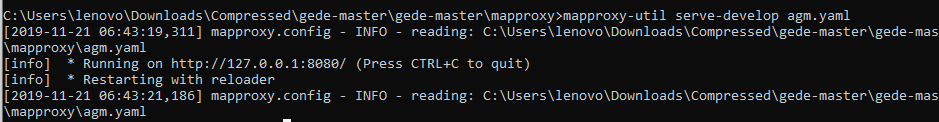
\includegraphics[width=12cm]{figures/Tugas5/1174071/1.png}
		\centering
		\caption{Run Mapproxy}
	\end{figure}
	
	\item Buka folder leafjs yang ada di folder gede, lalu buka file basic.html
    \hfill\break
    \begin{figure}[H]
		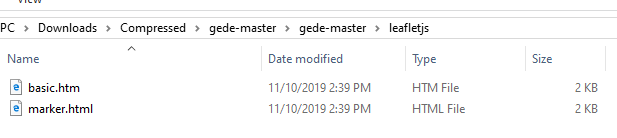
\includegraphics[width=12cm]{figures/Tugas5/1174071/2.png}
		\centering
		\caption{File basic.html}
	\end{figure}
	
	\item Buka file basic.html di browser, maka hasilnya akan seperti ini
    \hfill\break
    \begin{figure}[H]
		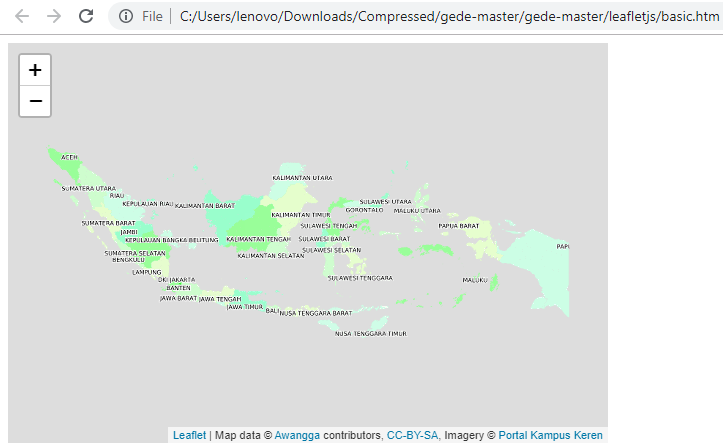
\includegraphics[width=12cm]{figures/Tugas5/1174071/3.png}
		\centering
		\caption{Hasil basic.html}
	\end{figure}
	
	\item Dengan leafletjs kita juga dapat menambahkan marker,circle, ataupun polygon dengan cara menggunakan L.marker, L.circle,  dan L.polygon. Contohnya file marker.html
    \hfill\break
	
	\item Buka file marker.html di text editor
    \hfill\break
	\begin{figure}[H]
		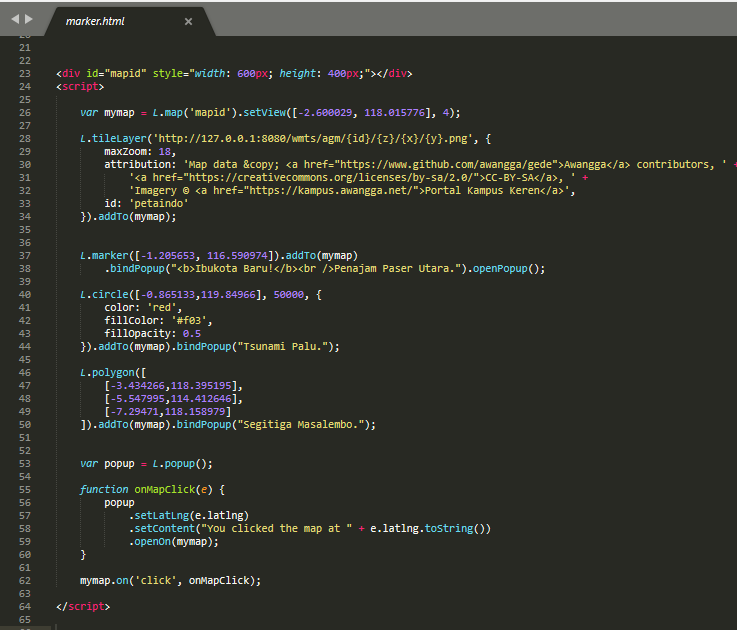
\includegraphics[width=12cm]{figures/Tugas5/1174071/4.png}
		\centering
		\caption{Kode untuk menggunakan marker, circle, dan polygon}
	\end{figure}

	\item Lalu buka file marker.html di web browser, dan seperti ini hasilnya
    \hfill\break
	\begin{figure}[H]
		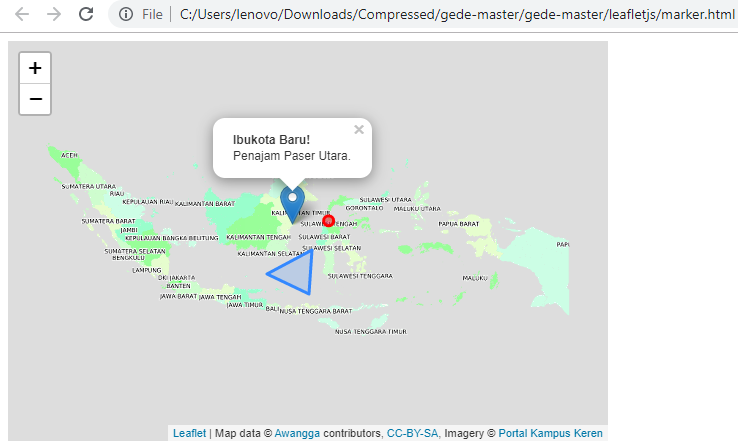
\includegraphics[width=12cm]{figures/Tugas5/1174071/5.png}
		\centering
		\caption{Hasil marker.html}
	\end{figure}
\end{enumerate}

\subsection{Link}
\url{https://youtu.be/iucxbB81h1A}
  